%%%%%%%%%%%%%%%%%%%%%%%%%%%%%%%%%%%%%%%%%%%%%%%%%
%------ LaTeX-Template für Abschlussarbeiten, Prof. Thomas Görne, Dezember 2012 --------
%%%%%%%%%%%%%%%%%%%%%%%%%%%%%%%%%%%%%%%%%%%%%%%%%

%---- Header (mit Formateinstellugen) laden, Inputencoding prüfen ------

%%%%%%%%%%%%%%%%%%%%%%%%%%%%%%%%%%%%%%%%%%%%%%%%%
%---- LaTeX-Header fuer Abschlussarbeiten, Prof. Thomas Goerne, Dez. 2012/Aug. 2013 ----
%%%%%%%%%%%%%%%%%%%%%%%%%%%%%%%%%%%%%%%%%%%%%%%%%

\documentclass[12pt,paper=A4,pointlessnumbers,bibtotoc,liststotoc,DIV=11,BCOR=1mm]{scrreprt}
% BCOR ist die Bindekorrektur (verlorener Rand am linken Blattrand)! Wert haengt von der Art der Heftung ab!!
% DIV ist eine Satzspiegeleinstellung von KOMA-Script / sccreprt.

\pagestyle{headings}

\usepackage[T1]{fontenc} % Font Encoding fuer europaeische Schriften mit Umlauten (Unterstuetzung der Worttrennung)
\usepackage{lmodern} % PostScript-Varianten der TeX Computer Modern-Schriften laden
\usepackage[english,ngerman]{babel} % Spracheinstellungen fuer Englisch und Neudeutsch laden

\usepackage{graphicx} % Grafikeinbindung (fuer .JPG, .JPEG, .PNG und .PDF, falls pdflatex benutzt wird)
\usepackage[table]{xcolor} % ermoeglicht farbige Schrift und farbige Tabellenzeilen
\definecolor{black}{gray}{0} % Umdefinition der Farbe black, falls noetig (0=schwarz, 1=weiss)
\definecolor{dblue}{rgb}{0.1,0.2,0.6} % Dunkelblau, fuer Hyperlinks
\definecolor{lgray}{gray}{0.9} % Hellgrau, fuer Tabellen (0=schwarz, 1=weiss)

\usepackage{booktabs} % fuer schoene Tabellen

\usepackage[round,authoryear]{natbib} % Literaturverweise mit Name/Jahreszahl in runden Klammern
\bibpunct[:\,]{(}{)}{,}{a}{}{,~}  % Feinformatierung der Natbib-Zitierweise

\usepackage[hyphens]{url}
\usepackage[colorlinks=true,linkcolor=black,citecolor=dblue,urlcolor=dblue]{hyperref} 
\usepackage{hyperref}  
% die Pakete url und hyperref ermoeglichen anklickbare URLs im Quellenverzeichnis in definierter Farbe, 
% sie ermoeglichen den Zeilenumbruch bei langen URLs, und sie erzeugen Hyperlinks (Farbe s.o.) 
% zwischen Quellenverweis und Quellenverzeichnis sowie zwischen label und ref im PDF-Dokument

% Fonteinstellungen fuer Bildunterschriften: Unterschrift serifenlos, "Abbildung" fett (bfseries = bold face series)
\setkomafont{captionlabel}{\sffamily\bfseries}
\setkomafont{caption}{\sffamily}

%------------------------------------------------------------------------------------------------------------------
%------ Eigenstaendigkeitserklaerung im gerahmten Kasten (parbox in einer framebox) ------
%------------------------------------------------------------------------------------------------------------------

\newcommand{\eigen}{
\setlength{\fboxsep}{2ex}
\setlength{\fboxrule}{0.8pt} 
% Einstellungen fuer Rahmenabstand und Rahmendicke der Framebox
\begin{center}
	\fbox{
		\parbox{0.8\linewidth}{
		Ich versichere, die vorliegende Arbeit selbstst\"andig ohne fremde Hilfe verfasst 
		und keine anderen Quellen und Hilfsmittel als die angegebenen benutzt zu haben. 
		Die aus anderen Werken w\"ortlich entnommenen Stellen oder dem Sinn nach 
		entlehnten Passagen sind durch Quellenangaben eindeutig kenntlich gemacht.
		\par\bigskip\bigskip\bigskip\bigskip
		\hspace*{0.8cm}Ort, Datum \hfill \vorname~\nachname\hspace*{0.8cm}
		}
	}
\end{center}
}

%%%%%%%%%%%%%%%%%%%%%%%%%%%%%%%%%%%%%%%%%%%%%%%%%


%------------------------ Titelblatt-Layout laden ----------------------------------

%%%%%%%%%%%%%%%%%%%%%%%%%%%%%%%%%%%%%%%%%%%%%%%%%
%------ LaTeX-Titelblatt fuer Bachelorarbeiten, Prof. Thomas Goerne, Dezember 2012 -------
%------------------------------------------------------------------------------------------------------------------
%--------------------------------- Deklarationen fuer die Titelseite  --------------------------------------
%%%%%%%%%%%%%%%%%%%%%%%%%%%%%%%%%%%%%%%%%%%%%%%%%

\title{\titel\\[2ex]
\LARGE Bachelor-Thesis\\
\large zur Erlangung des akademischen Grades B.Sc.\\[1.5ex]
\LARGE \vorname~\nachname\\[0.5ex] 
\large \matrikelnummer
}

\author{\unitlength1mm
\large\raisebox{-1ex}{
\includegraphics[width=4em]{HAW_wuerfel}}\hspace{1ex}
\parbox[b]{11.2cm}{\sffamily\large%
Hochschule f\"ur Angewandte Wissenschaften Hamburg\\[-0.2ex]
Fakult\"at Design, Medien und Information\\[-0.2ex]
Department Medientechnik
}\\[6ex]
\sffamily\large Erstpr\"ufer: \erstpruef\\[0.5ex]
\sffamily\large Zweitpr\"ufer: \zweitpruef}

%%%%%%%%%%%%%%%%%%%%%%%%%%%%%%%%%%%%%%%%%%%%%%%%%
%\input{hawmt-master-titelblatt}

%---------------------------- Titeldefinitionen --------------------------------------

\newcommand{\vorname}{Matthias}
\newcommand{\nachname}{Held}
\newcommand{\matrikelnummer}{2182712}

\newcommand{\titel}{\glqq Red Tail\grqq\ :\\ Auswirkung eines zusätzlichen tiefroten Spektralanteils auf das Weißlicht von LED-Scheinwerfern\\[0.2ex] 
				\Large - am Beispiel der Beleuchtung von Hauttönen im TV-Bereich}

\newcommand{\erstpruef}{Prof. Dr. Roland Greule}
\newcommand{\zweitpruef}{Dipl. Ing. (FH) Matthias Allhoff}

\date{vorläufige Fassung vom \today}   % praktisch für Vorab-Versionen. 
%\date{\sffamily Hamburg, 2. 2. 2020}  % Abgabedatum!

%--------------------------------------------------------------------------------------
%----------------------------- hier gehts los! --------------------------------------
%--------------------------------------------------------------------------------------

\begin{document}
\selectlanguage{ngerman}
\maketitle           % Titelseite erzeugen
\tableofcontents % Inhaltsverzeichnis erzeugen
\clearpage          % Seitenumbruch


%------------ Zusammenfassung / Abstract ------------------

\thispagestyle{empty}
\selectlanguage{english}
\section*{\centering\abstractname}
Form and layout of this \LaTeX-template incorporate the guidelines for theses in the Media Technology Department \glqq Richtlinien zur Erstellung schriftlicher Arbeiten, vorrangig Bachelor-Thesis (BA) und Master-Thesis (MA) im Department Medientechnik in der Fa\-kul\-t{\"a}t DMI an der HAW Hamburg\grqq\ in the version of December 6, 2012 by Prof.\ Wolfgang Willaschek. 

The thesis should be printed single-sided (simplex). The binding correction (loss at the left aper edge due to binding) might be adjusted, according to the type of binding. This template incorporates a binding correction as BCOR=1mm (suitable for adhesive binding) in the \LaTeX\ document header.

{\bfseries This is the english version of the opening abstract} (don't forget to set \LaTeX's language setting back to ngerman after the english text). 
 
 
\selectlanguage{ngerman}
\section*{\centering\abstractname}

Diese Arbeit befasst sich mit der Auswirkung eines zusätzlichen tiefroten Spektralanteils auf das kaltweiße Lichtspektrum von LED-Scheinwerfern. Es soll dabei überprüft werden, ob Personen unter diesen Umständen im Kamerabild natürlicher aussehen, wie es in der \glqq Red Tail\grqq\ - Theorie der mo2 design GmbH angenommen wird.\\
Zunächst wird auf wichtige Kenngrößen der Lichttechnik eingegangen und verschiedene Leuchtmittel und lichttechnische Parameter werden erläutert. Im Folgeneden werden die Messungen beschrieben.\\
Bei diesen wird ein LED-Scheinwerfer und ein rotgefilterter PAR-Scheinwerfer, der den\glqq Red Tail\grqq\ simulieren soll, auf einen Messpunkt ausgerichtet. Der LED-Scheinwerfer wird zuerst allein auf eine kaltweiße Referenzlichtquelle bestmöglich abgeglichen und spektral vermessen. Anschließend wird der rotgefilterter PAR-Scheinwerfer dazugeschlatet und auch dieses Lichtgemisch wird auf die Referenzlichtquelle abgeglichen und spektral vermessen. 
Bei der Auswertung werden die gemessenen lichttechnischen Parameter betrachtet und zusätzlich werden bei einer Umfrage Bilder verglichen, auf denen Probanden verschiedener Hauttöne mit und ohne \glqq Red Tail\grqq\ beleuchtet wurden.




%--------------------------- Text -------------------------------

\chapter{Einleitung}

\section{Unterkapitel mit Mathematik, Bildern und Querverweisen}


\chapter{Grundlagen und Kenngrößen der Lichttechnik}



\section{Wie sehen wir Licht} \label{sec_wiesehenwir}
Für den Menschen sind elektromagnetische Wellenlänge im Bereich von 380nm - 780nm sichtbar (Abb. \ref{b_sichtbareslicht}). 

\begin{figure}[htp]     % h=here, t=top, b=bottom, p=page
\centering
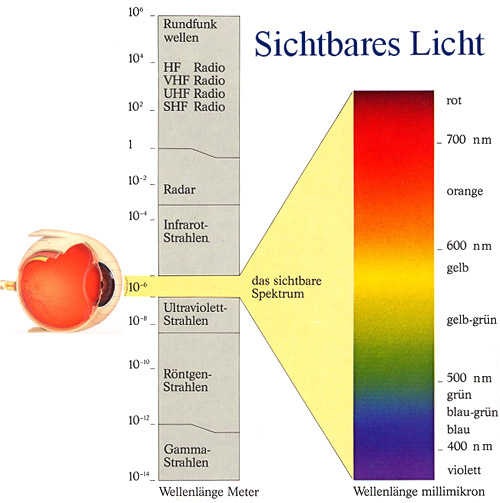
\includegraphics[width=0.7\textwidth]{bilder/sichtbares_licht} 
% Bilddatei aus dem Unterverzeichnis bilder holen, skalieren auf 0.8*Satzspiegel
\caption {Für das menschliche Auge sichtbarer Bereich des elektromagnetischen Spektrums\protect\footnotemark}\label{b_sichtbareslicht}
\end{figure}

\footnotetext{\url{https://www.allmystery.de/i/t4f0016_sichtbares_licht.jpg}}

Ein Selbstleuchter ist eine natürliche oder künstliche Lichtquelle, die Licht im sichtbaren Bereich emittiert. Körperfarben hingegen entstehen durch Reflexion oder Transmission von Licht auf einen nichtselbstleuchtenden Gegenstand. Bei der Beobachtung der Körperfarben hinsichtlich ihrer Beleuchtung wird die Farbewiedergabe des Lichts bestimmt\citep[S.103]{hentschel}.



\section{test}

\section{Farben und Farbmischungen}
Eine Farbe kann mit den drei Bestimmungsstücken Helligkeit, Farbton und Sättigung beschrieben werden. Die Helligkeit wird als Äquivalent zu der Leuchtdichte bei Selbstleuchtern (zum Leuchtedichtefaktor bei Körperfarben) gesehen. Die empfundene Helligkeit von Licht ist immer durch die V($\lambda$)-Kurve bewertet (siehe Abschnitt\ref{sec_wiesehenwir}).
Der Farbton ist das Äquivalent der Farbempfindung. Mit ihm wird ausgedrückt, welcher Farbname der Farbe zugeordnet wird.
Die Sättigung bestimmt wie groß der Anteil eines Farbtons einer Farbe ist. Weiß und Schwarz haben eine Sättigung von 0 und werden daher unbunte Farben genannt \citep[S.102-103]{hentschel}.


Für die additive Farbmischung gelten nach Grassmann (1853) folgende drei Regeln:

\begin{enumerate}\setlength{\itemsep}{0ex}
\item Für das Ergebnis einer additiven Farbmischung ist nur das Aussehen, nicht die spektrale Zusammensetzung der Komponenten maßgebend.
\item Alle Farbmischungen verlaufen stetig.
\item Zum Festlegen einer Farbe sind drei Bestimmungsstücke notwendig und hinreichend 
\end{enumerate}

Die erste Regel bedeutet, dass das bloße Auge nicht erkennen kann aus welchen sprektralen Komponenten Licht besteht. Ein orangenes Licht einer amberfarbenen LED kann (bei gleicher Helligkeit, Farbton und Sättigung) nicht von einem orangen Licht unterschieden werden, dass aus einer roten und einer grünen LED gemischt wurde.

\begin{figure}[htp]     % h=here, t=top, b=bottom, p=page
\centering
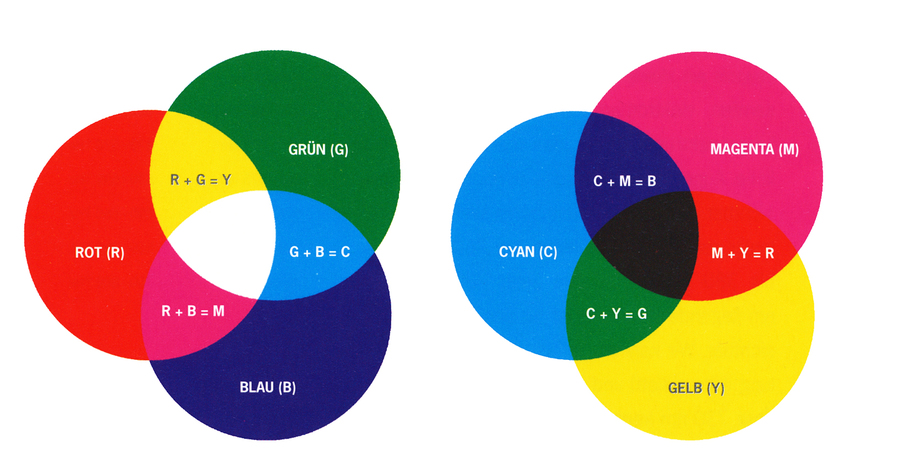
\includegraphics[width=0.7\textwidth]{bilder/additve_und_subtraktive_Farben} 
% Bilddatei aus dem Unterverzeichnis bilder holen, skalieren auf 0.8*Satzspiegel
\caption {Additive Farbmischung mit rot, grün und blau (l.) und Subtraktive Farbmischung mit cyan, magenta und gelb (r.) \protect\footnotemark}
\end{figure}

\footnotetext{\url{https://www.axel-venn.de/s/cc_images/teaserbox_23365996.jpg?t=1415014980}}



Die Gesichtsempfindung "Farbe" entsteht durch Lichtreize von Selbstleuchtern oder Körperfarben. Um eine solche Farbe zu beschreiben sind nach dem 3. Graßmannschen Satz \emph{\glqq drei Bestimmungsstücke notwendig und ausreichend\grqq} \citep[S.102-103]{hentschel}

\section{Farbräume}

\chapter{Messungen}

\section{Unterkapitel mit Mathematik, Bildern und Querverweisen}

\chapter{Messergebnisse}

\section{Unterkapitel mit Mathematik, Bildern und Querverweisen}

\chapter{Umfrage}

\section{Unterkapitel mit Mathematik, Bildern und Querverweisen}

\chapter{Umfrageergebnisse}

\section{Unterkapitel mit Mathematik, Bildern und Querverweisen}

\chapter{Auswertung aller Ergebnisse}

\section{Unterkapitel mit Mathematik, Bildern und Querverweisen}

\chapter{Fazit}

\section{Unterkapitel mit Mathematik, Bildern und Querverweisen}





%--------------------- VERZEICHNISSE ----------------

\listoffigures % Abbildungsverzeichnis erzeugen
\listoftables % Tabellenverzeichnis erzeugen

%--------------------- LITERATURLISTE ---------------
% Die Einträge sollen alphabetisch sortiert sein.

\begin{thebibliography}{}

% Formatierung für Internetquelle
% Grundregel: Name, Vorname (falls vorhanden), VÖ-Jahr (falls vorhanden), Titel in Anführungszeichen, URL, Datum des letzten Aufrufs
% zur Formatierung der URL unbedingt den url-Befehl benutzen!!!

\bibitem[Production Partner(2018)]{production partner}
Production Partner:
\emph{\glqq Farbwiedergabe: TM-30-15, CRI und Co.\glqq}
\url{https://www.production-partner.de/basics/farbwiedergabe-tm-30-15-cri-und-co/}, 22.02.2018, letzter Zugriff 20.06.2018


\bibitem[Gigahertz-Optik(2012)]{Gigahertz}
Gigahertz-Optik:
\emph{\glqq Grundladen der Lichtmesstechnik\grqq}
\url{https://www.gigahertz-optik.de/de-de/grundlagen-lichtmesstechnik/}, letzter Zugriff 20.06.2018


% Formatierung für Aufsatz / Paper: Titel in Anführungszeichen, Zeitschriftentitel kursiv
\bibitem[Dooley \& Streicher(1982)]{dooley_streicher} 
Dooley, Wesley L.  \& Streicher, Ronald D.:
\glqq M--S Stereo: A Powerful Technique for Working in Stereo\grqq, 
\emph{Journ. Audio Engineering Society} vol. 30 (10), 1982

% Formatierung für Fachbuch, Diplomarbeit o.Ä.: Titel kursiv

\bibitem[Hentschel(1993)]{hentschel}
Hentschel, Hans-Jürgen: 
\emph{Licht und Beleuchtung Theorie und Praxis der Lichttechnik}, 4. Aufl., Hüthig 1994

% Formatierung für Fachbuch mit Herausgeber und mehreren Autoren
\bibitem[Spehr(2009)]{spehr}
Spehr, Georg (Hrsg.): 
\emph{Funktionale Klänge}, transcript 2009

\bibitem[Greule(2014)]{greule}
Greule, Roland (Autor):
\emph{Licht und Beleuchtung im Medienbereich}, Hanser 2015 


% Formatierung für ein einzelnes Kapitel eines speziellen Autors aus einem Fachbuch mit mehreren Autoren
\bibitem[Sowodniok(2009)]{sowodniok}
Sowodniok, Ulrike: 
\glqq Funktionaler Stimmklang -- Ein Prozess mit Nachhalligkeit\grqq, 
in: Spehr, Georg (Hrsg.): \emph{Funktionale Klänge}, transcript 2009




% Formatierung für Aufsatz / Paper: Titel in Anführungszeichen, Zeitschriftentitel kursiv
\bibitem[Stephenson(1990)]{stephenson}
Stephenson, Uwe: 
\glqq Comparison of the Mirror Image Source Method and the Sound Particle Simulation Method\grqq, 
\emph{Applied Acoustics} vol. 29, 1990


\end{thebibliography}

%--------------------- EIGENSTÄNDIGKEITSERKLÄRUNG ---------------
\clearpage\thispagestyle{empty}
\eigen  % im header definiert
%--------------------------------------- ENDE ------------------------------------
\end{document}
%%%%%%%%%%%%%%%%%%%%%%%%%%%%%%%%%%%%











